\comment{Suggestion: past tense}\\

\subsection{Gradient Descent Analysis}
    First we looked at our library of gradient descent methods to figure out what and how they worked. This with the goal of finding a descent recipe for optimising our neural networks down the line.
    
    \subsubsection{OLS Optimisation}
        All plots regarding the optimisation of the OLS cost function are found in \cref{res:fig:lrates}. The best MSE scores and learning rates are tabulated in \cref{res:tab:OLS_MSEs}. We found that the none of the algorithms come really close to the analytical OLS solution, found by matrix inversion, with a validation MSE of $0.1176$. The best performing algorithms were SGD with Adam (MSE $0.1660 \pm 0.0018$), SGD with momentum (MSE $0.1729 \pm 0.0022$) and GD with momentum (MSE $0.1775 \pm 0.0026$).

        In \cref{res:fig:lrate1} we see that both the non-stochastic and stochastic algorithms performed better when momentum was added, which helped avoid local minima to converge faster and prevent exploding gradients. Generally, the stochastic algorithms had tighter confidence intervals, signalling that they are not as sensitive to the initial conditions as the plain algorithms.

        Exploring the increase in epochs and decrease in batch size in \cref{res:fig:lrate2}, we see that decreasing batch size made the algorithm less stable, and more easily prone to exploding gradients. Increasing the number of epochs improved the result, and made increased the convergence, but did not affect stability.

        Adding the tuning of the learning rate with AdaGrad, we see in \cref{res:fig:lrate3} a marked increase in stability. However, the algorithms struggled to converge, with the momentum based algorithms doing best, SGD slightly bettering the GD results. However, even AdaGrad SGD with momentum could not beat the ordinary momentum based GD and SGD algorithms.

        Introducing RMSprop and Adam to tune the learning rate provided algorithms with a tunable learning rate that converged faster than AdaGrad, seen in \cref{res:fig:lrate4}. Instead of exploding, the MSE of RMSprop gradually increased from around $\eta=0.1$. Ultimately, it performed similarly to the AdaGrad algorithms, with an optimal MSE of 0.1863. The momentum based Adam algorithm performed the best, with an optimal MSE of $0.1660$; but performing well from very low $\eta$-values up to around $\eta=0.35$. After this point Adam was markedly less stable than the AdaGrad algorithms. Aside from converging faster, it was also notable that both RMSprop and Adam were much less sensitive to initial conditions, with generally much tighter confidence intervals. \network{1}{2}

        \begin{table}[!ht]
            \centering
            \begin{tabular}{r|c|l}
                Method & MSE & $\eta$ \\ \hline
                Analytic & 0.1377 & - \\
                Plain GD & $0.1982 \pm 0.0061$ & 0.072 \\
                Momentum GD & $0.1775 \pm 0.0026$ & 0.13 \\
                Plain SGD & $0.1862 \pm 0.0028$ & 0.069 \\
                Momentum SGD & $0.1729 \pm 0.0022$ & 0.12 \\
                AdaGrad GD & $0.2135 \pm 0.012$ & 0.50 \\
                AdaGrad Momentum GD & $0.1836 \pm 0.0024$ & 0.52 \\
                AdaGrad SGD & $0.1906 \pm 0.0038$ & 0.50 \\
                AdaGrad Momentum SGD & $0.1822 \pm 0.0020$ & 0.47 \\
                RMSprop SGD & $0.1859 \pm 0.0027$ & 0.019 \\
                Adam SGD & $0.1660 \pm 0.0018$& 0.32 \\
            \end{tabular}
            \caption{Table of the best validation MSE scores by GD algorithm, together with the learning rate that produced the best result.}
            \label[tab]{res:tab:OLS_MSEs}
        \end{table}

        \begin{figure*}
            \begin{subfigure}{.49\textwidth}
                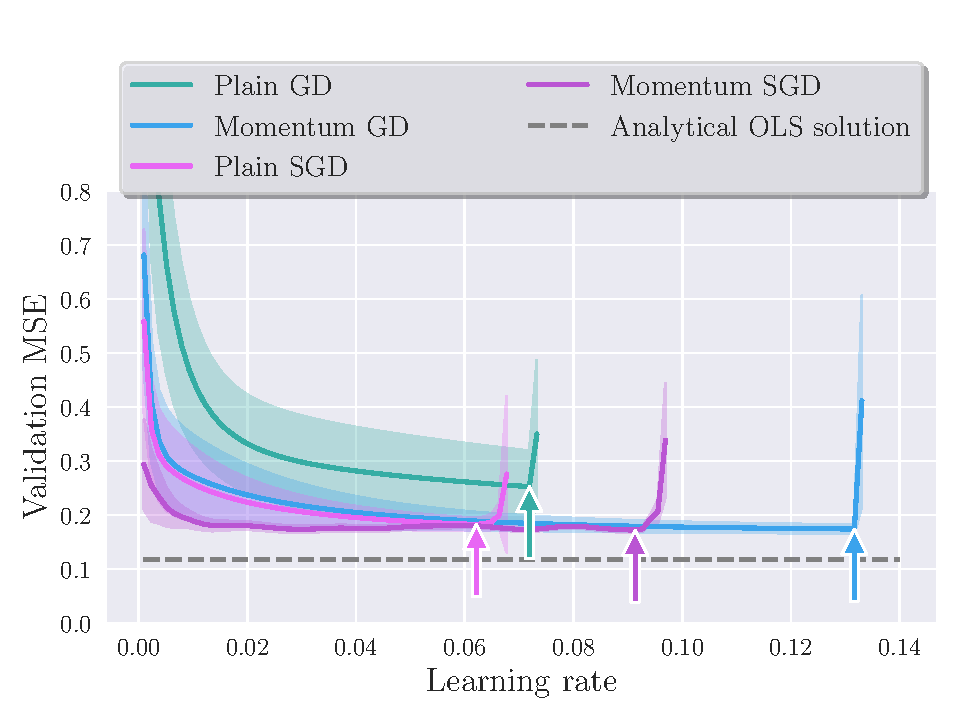
\includegraphics[width=\linewidth]{learning_rates_PGD_MGD_PSGD_MSGD.pdf}
                \caption{The minimal MSEs by algorithm: plain GD 0.1982 ($\eta=0.072$), GD w/momentum 0.1775 ($\eta=0.13$), plain SGD 0.1862 ($\eta=0.069$), SGD w/momentum 0.1729 ($\eta=0.12$)}
                \label[fig]{res:fig:lrate1}
            \end{subfigure}
            \hfill
            \begin{subfigure}{.49\textwidth}
                \centering
                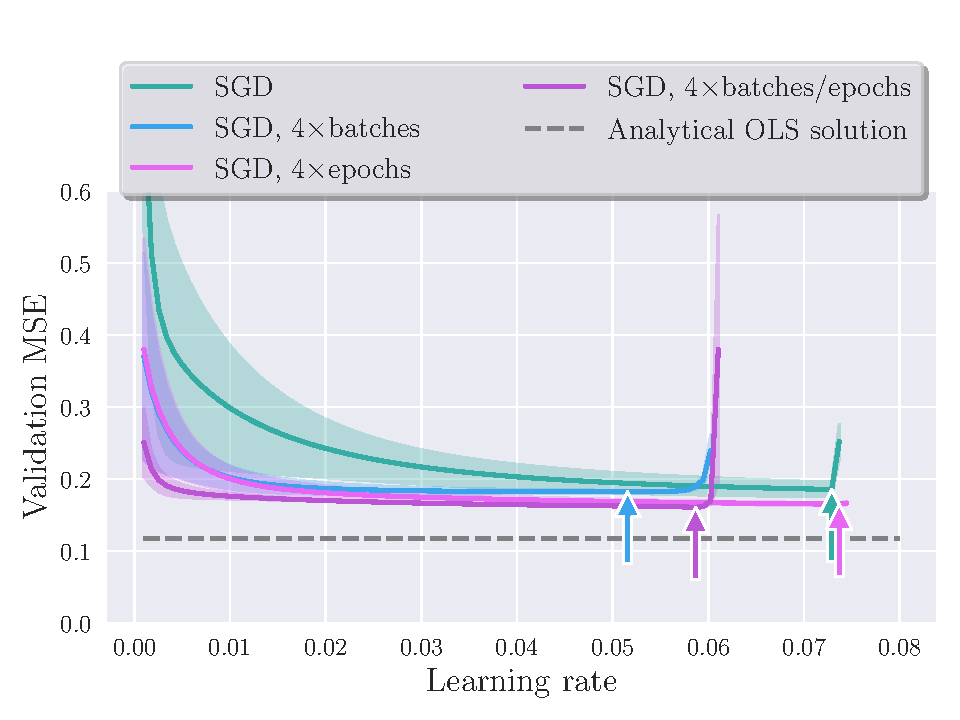
\includegraphics[width=\linewidth]{learning_rates_SGD_batches_epochs.pdf}
                \caption{The minimal MSEs of plain SGD by number of epochs and batch size: 500 epochs/200 batch size 0.1862 ($\eta=0.068$), 500 epochs/50 batch size 0.1819 ($\eta=0.0026$), 2000 epochs/64 batch size 0.1776 ($\eta=0.071$), 2000 epochs/50 batch size 0.1773 ($\eta=0.057$)}
                \label[fig]{res:fig:lrate2}
            \end{subfigure}
            \hfill
            \begin{subfigure}{.49\textwidth}
                \centering
                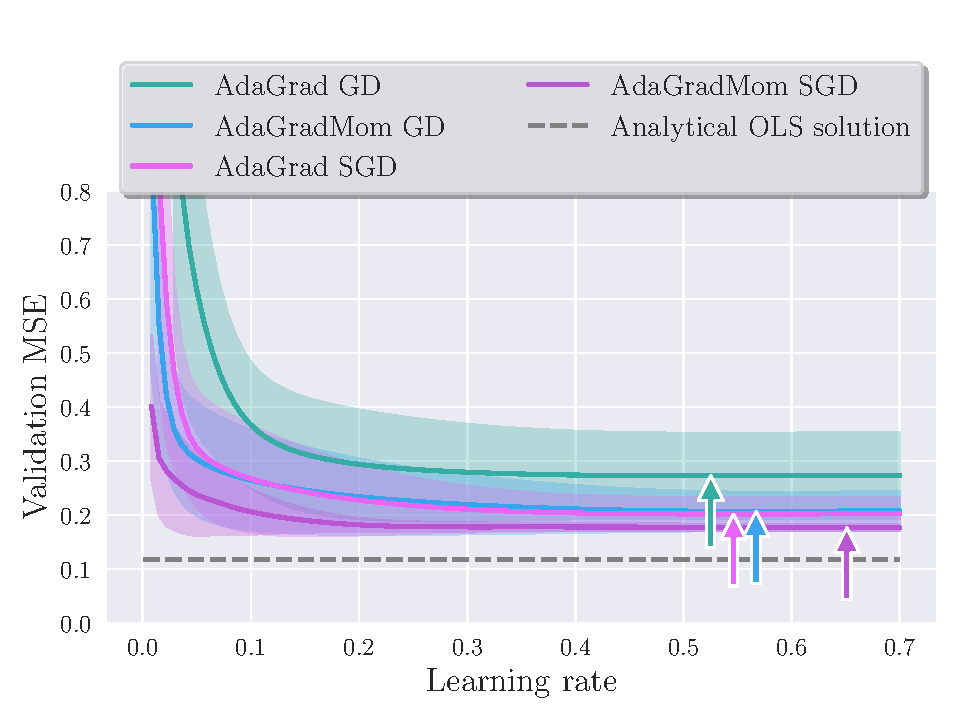
\includegraphics[width=\linewidth]{learning_rates_adagrad}
                \caption{The minimal MSEs by algorithm: AdaGrad GD 0.2135 ($\eta=0.50$), AdaGrad GD w/momentum 0.1836 ($\eta=0.52$), AdaGrad SGD 0.1906 ($\eta=0.50$), AdaGrad SGD w/momentum 0.1822 ($\eta=0.47$)}
                \label[fig]{res:fig:lrate3}
            \end{subfigure}
            \hfill
            \begin{subfigure}{.49\textwidth}
                \centering
                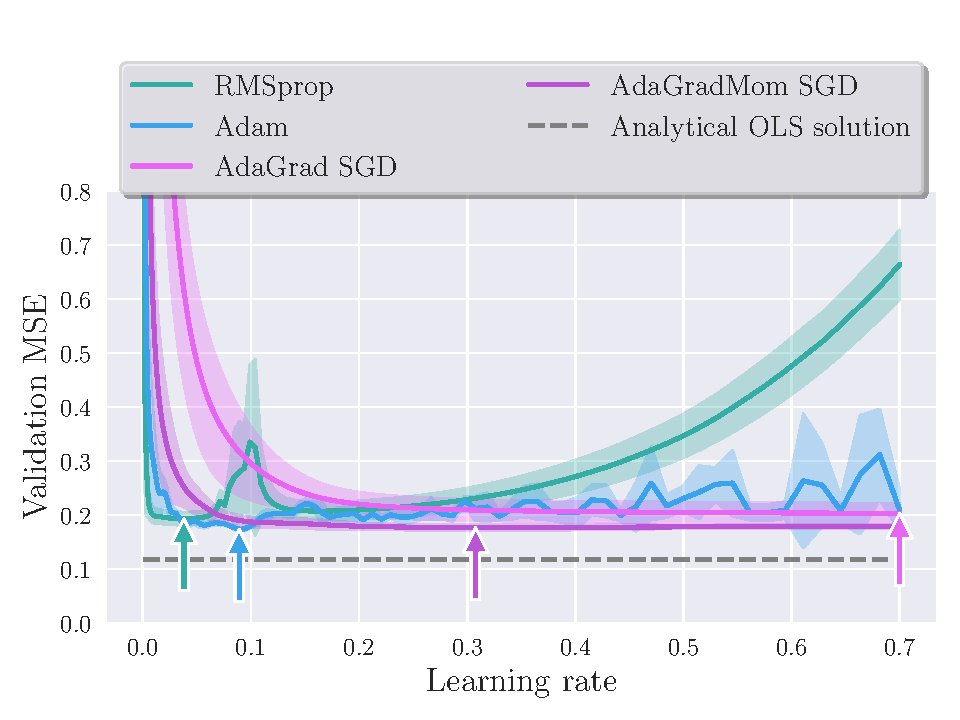
\includegraphics[width=\linewidth]{learning_rates_tunable}
                \caption{The minimal MSEs by algorithm: RMSprop SGD 0.1859 ($\eta=0.019$), Adam SGD 0.1660 ($\eta=0.32$), AdaGrad SGD 0.1906 ($\eta=0.50$), AdaGrad SGD w/momentum 0.1823 ($\eta=0.46$)}
                \label[fig]{res:fig:lrate4}
            \end{subfigure}
            \caption{Plots of the validation MSE of the parameters found from optimising the OLS cost function on Franke function data with $n=600$ data points with a train test split of $\sfrac{3}{4}$. For the momentum methods we used $\gamma=0.8$, for RMSprop we used $\beta=0.9$ and for Adam we used $\beta_1=0.9, \beta_2=0.99$. The stochastic methods used a batch size of 200 and 500 epochs, while the standard GD did 500 iterations unless specified otherwise. Overlaid are 95\% confidence intervals based on optimising with five different starting points. Exploded gradients are clipped out of the plot. The analytical OLS solution achieved an MSE of 0.1377.}
            \label[fig]{res:fig:lrates}
        \end{figure*}

    \subsubsection{Ridge Optimisation}
        The results from the ridge analysis are found in \cref{res:fig:GDridge}, and a summary is tabulated in \cref{res:tab:ridge_MSEs}. 
        
        We did not see much change in the performance of the algorithms from the OLS optimisation. There was in fact a slight decrease in the optimal MSE of all the algorithms except AdaGrad with momentum, however, the std of the MSEs generally went down. There was no universal $\lambda$-value that gave the best results. It is worth noting that there was little effect on where the exploding gradients occur; in fact with larger $\lambda$-values they occur earlier for both GD and SGD with momentum.

        The best performing algorithm was again SGD with Adam to tune the learning rate (MSE of $0.1673 \pm 0.0020$), as before with the OLS cost function.

        To see whether ridge actually had the potential to do a difference, we plotted the validation MSE of the analytical ridge solution as a function $\lambda$ against the analytical OLS solution in \cref{res:fig:ridge_ana}. We see that the ridge solution does actually perform better than OLS between $\lambda \in [0.0001, 0.01]$, meaning that there is potential for improvement with the ridge penalisation.

        \begin{table}[ht!]
            \centering
            \scalebox{0.85}{
            \begin{tabular}{r|c|l|l}
                Method & MSE & $\eta$ & $\lambda$ \\ \hline
                Analytic & 0.1338 & - & 0.002 \\
                Momentum GD & $0.1777 \pm 0.0025$ & 0.13 & $10^{-4}$ \\
                Momentum SGD & $0.1747 \pm 0.0020$ & 0.12 & $10^{-8}$ \\
                AdaGrad Momentum SGD & $0.1822 \pm 0.0013$ & 0.48 & $10^{-3}$ \\
                Adam SGD & $0.1673 \pm 0.0020$ & 0.32 & $10^{-5}$
            \end{tabular}
            }
            \caption{Summary of the best validation MSEs resulting from the optimisation of the ridge cost function using various GD algorithms. The data is taken from the plots in \cref{res:fig:GDridge}.}
            \label[tab]{res:tab:ridge_MSEs}
        \end{table}

        \begin{figure*}
            \begin{subfigure}{.49\textwidth}
                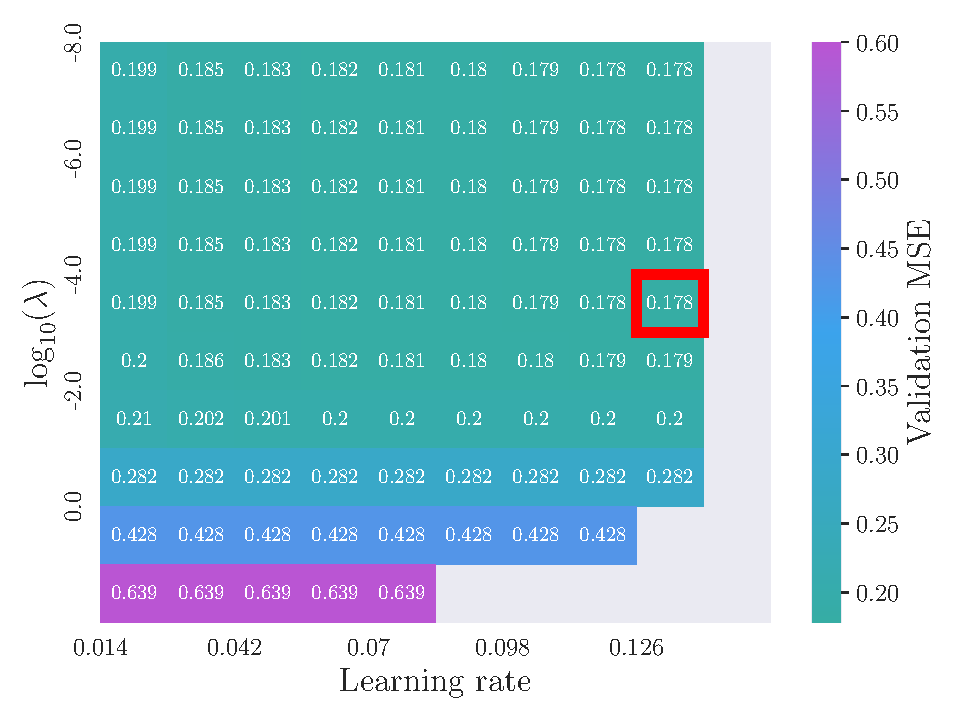
\includegraphics[width=\linewidth]{lmbda_learning_rates_momentum_GD.pdf}
                \caption{\textbf{GD with momentum}. Best MSE value was 0.1777 with $\lambda=10^{-4}, \eta=0.13$.}
                \label[fig]{res:fig:mGDridge}
            \end{subfigure}
            \hfill
            \begin{subfigure}{.49\textwidth}
                \centering
                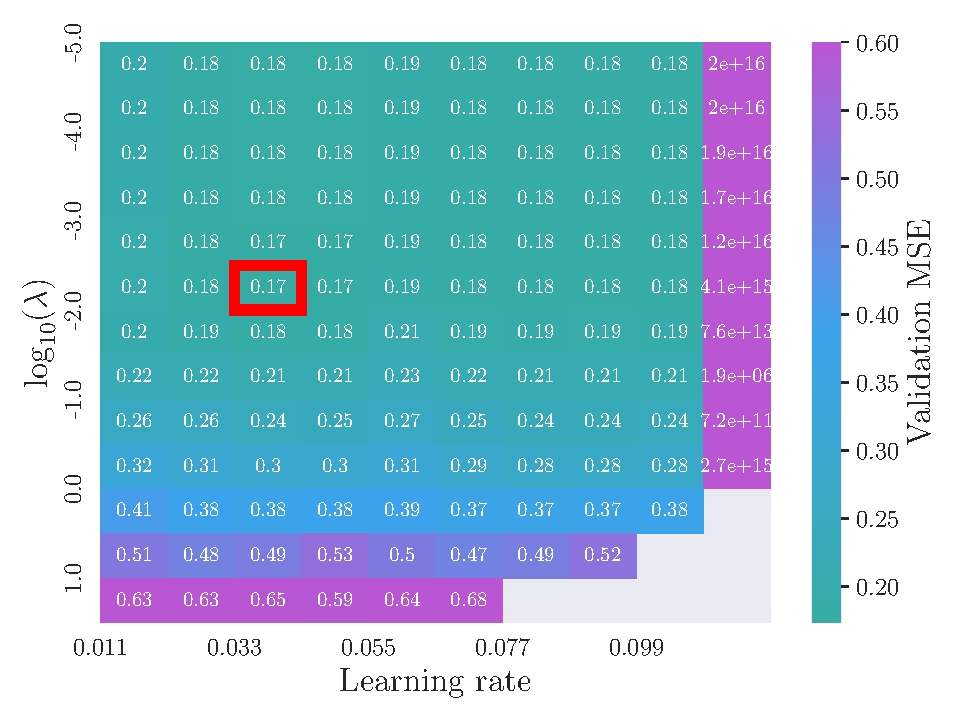
\includegraphics[width=\linewidth]{lmbda_learning_rates_momentum_SGD.pdf}
                \caption{\textbf{SGD with momentum}. Best MSE value was 0.1747 with $\lambda=10^{-8}, \eta=0.12$.}
                \label[fig]{res:fig:mSGDridge}
            \end{subfigure}
            \hfill
            \begin{subfigure}{.49\textwidth}
                \centering
                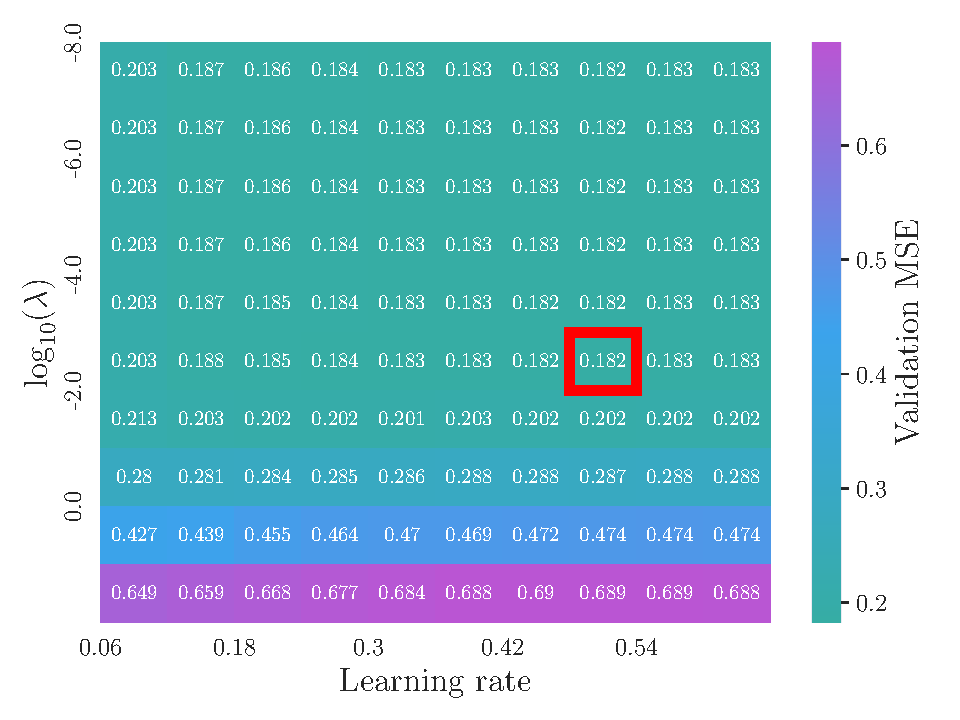
\includegraphics[width=\linewidth]{lmbda_learning_rates_adagrad_momentum_SGD.pdf}
                \caption{\textbf{SGD AdaGrad with momentum}. Best MSE value was 0.1822 with $\lambda=10^{-3}, \eta=0.48$.}
                \label[fig]{res:fig:agSGDridge}
            \end{subfigure}
            \hfill
            \begin{subfigure}{.49\textwidth}
                \centering
                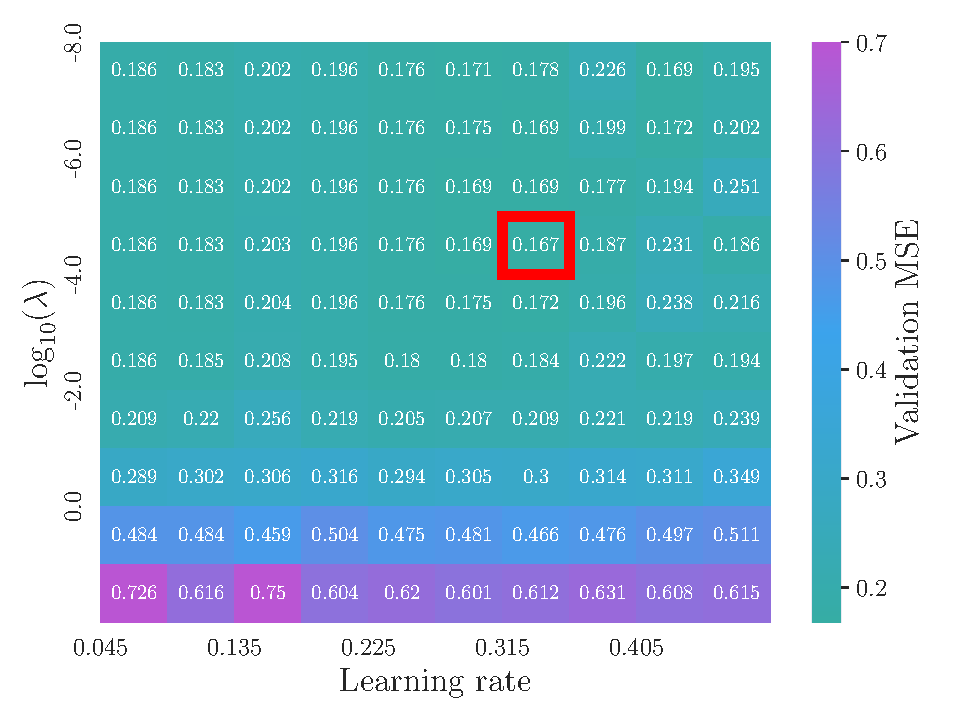
\includegraphics[width=\linewidth]{lmbda_learning_rates_adam_SGD.pdf}
                \caption{\textbf{SGD Adam}. Best MSE value was 0.1673 with $\lambda=10^{-5}, \eta=0.32$.}
                \label[fig]{res:fig:adSGDridge}
            \end{subfigure}
            \caption{Plots of the validation MSE of the parameters found from optimising the ridge cost function on Franke function data with $n=600$ data points with a train test split of $\sfrac{3}{4}$. For the momentum methods we used $\gamma=0.8$ and for Adam we used $\beta_1=0.9, \beta_2=0.99$. The stochastic methods used a batch size of 200 and 500 epochs, while the standard GD did 500 iterations unless specified otherwise. Overlaid are 95\% confidence intervals based on optimising with five different starting points. Exploded gradients are clipped out of the plot.}
            \label[fig]{res:fig:GDridge}
        \end{figure*}

        \begin{figure}[ht!]
            \centering
            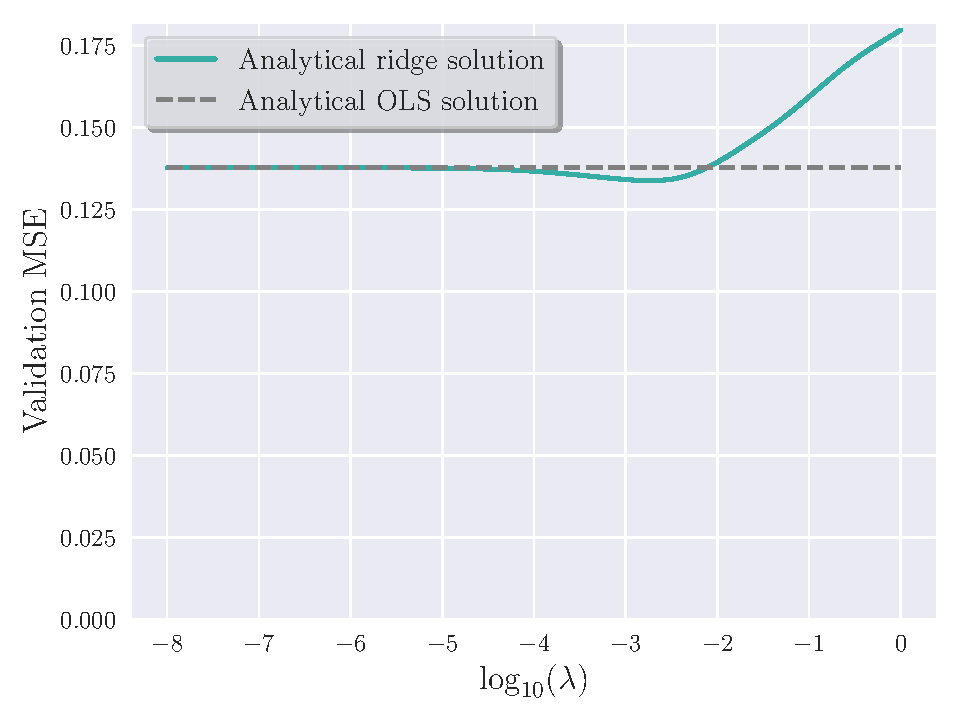
\includegraphics[width=\linewidth]{lmbda_plot_ana}
            \caption{Plot of the validation MSE found from optimising our linear regression parameters to the ridge cost function as a function of the penalisation parameter $\lambda$. The optimal MSE is 0.1338 with $\lambda = 0.002$.}
            \label[fig]{res:fig:ridge_ana}
        \end{figure}


\subsection{Neural Network and regression}
    \subsubsection{Network Structure}

        \begin{figure*}
            \begin{subfigure}{.49\textwidth}
                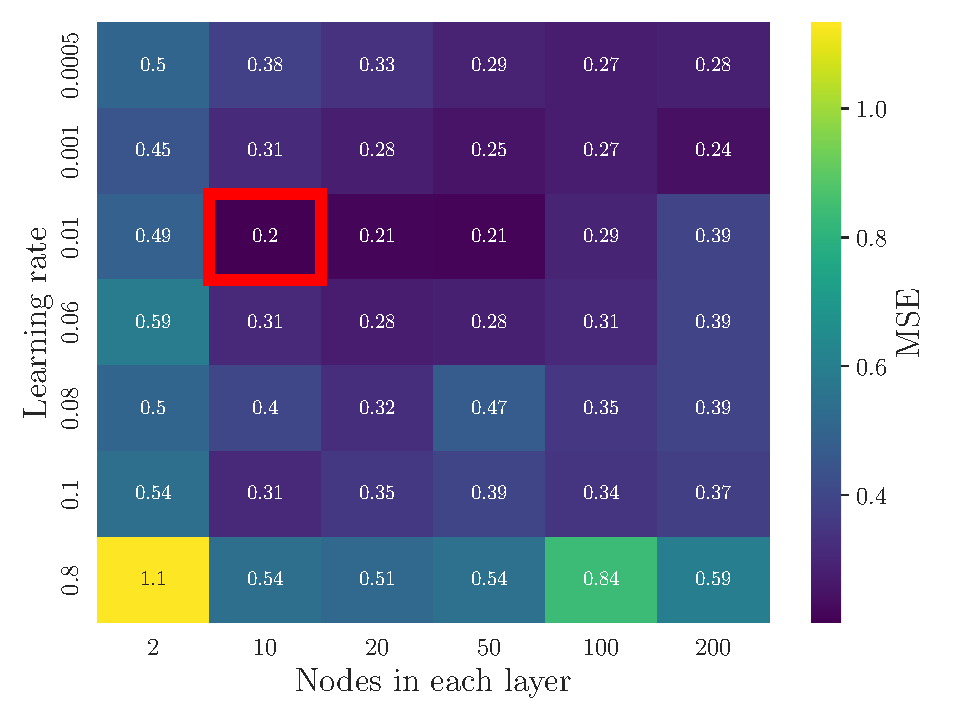
\includegraphics[width=\linewidth]{nodes_etas_heatmap_1.pdf}
                \caption{}
                \label[fig]{res:fig:1_lay}
            \end{subfigure}
            \hfill 
            \begin{subfigure}{.49\textwidth}
                \centering
                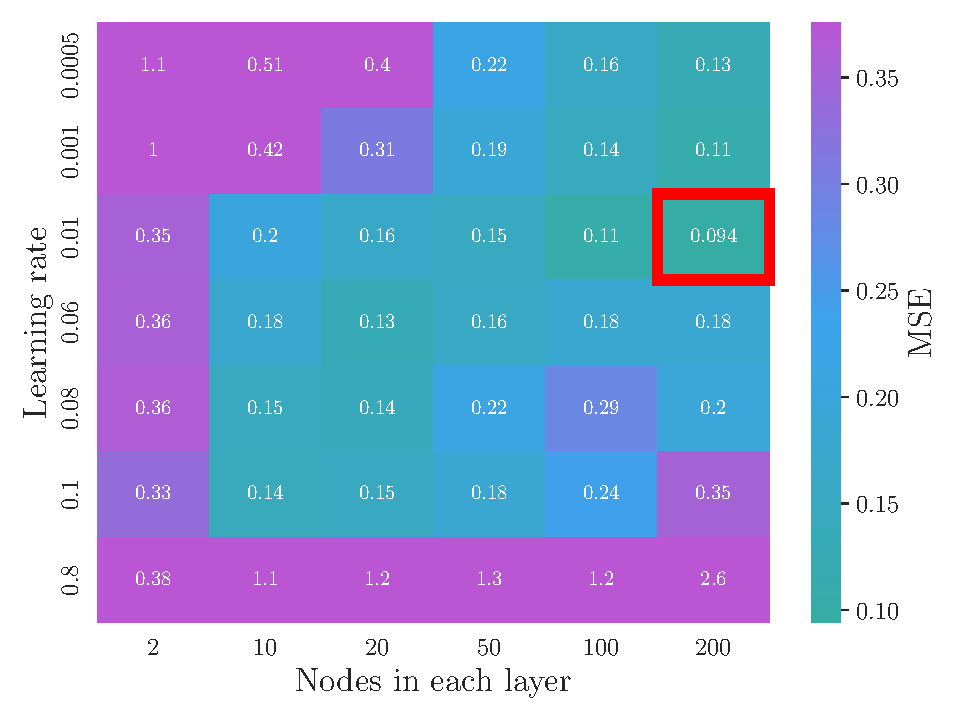
\includegraphics[width=\linewidth]{nodes_etas_heatmap_3.pdf}
                \caption{}
                \label[fig]{res:fig:3_lay}
            \end{subfigure}
            \hfill 
            \begin{subfigure}{.49\textwidth}
                \centering
                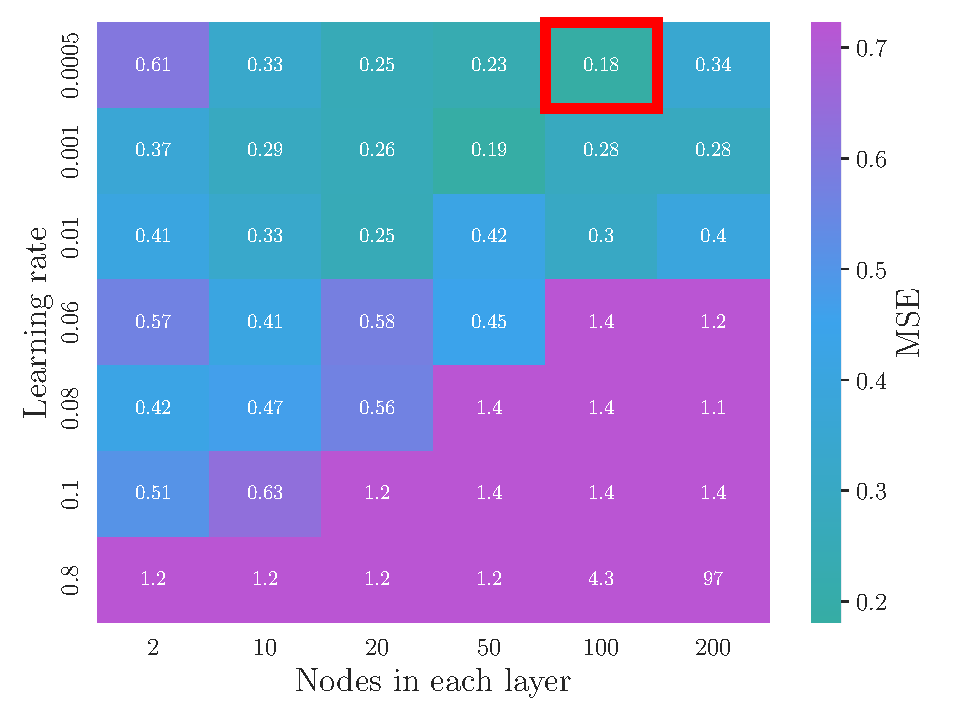
\includegraphics[width=\linewidth]{nodes_etas_heatmap_5.pdf}
                \caption{}
                \label[fig]{res:fig:5_lay}
            \end{subfigure}
            \hfill 
            \begin{subfigure}{.49\textwidth}
                \centering
                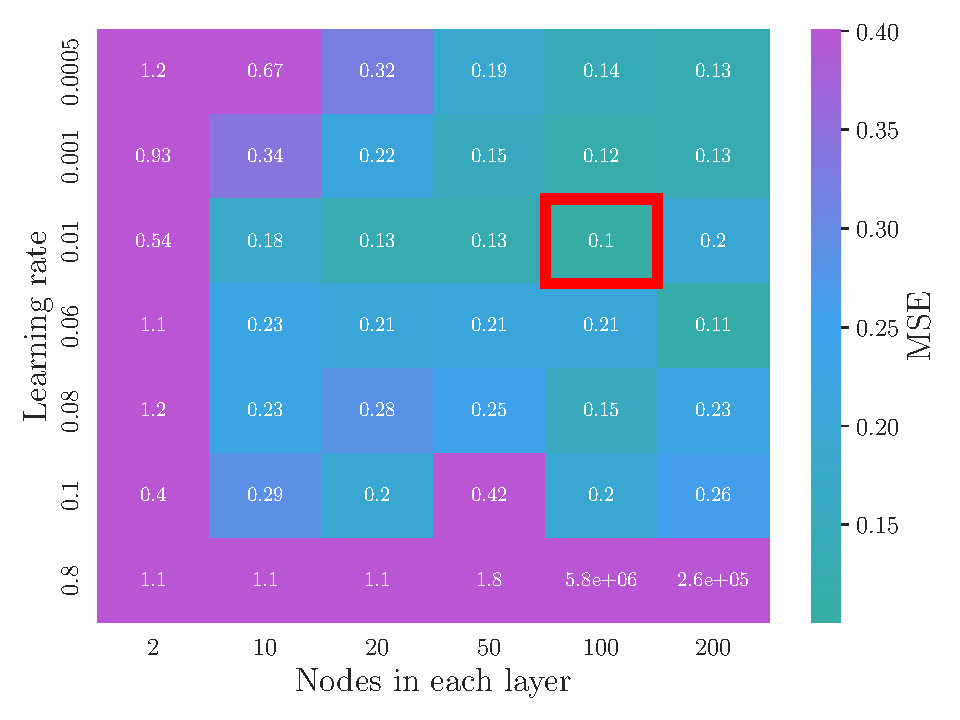
\includegraphics[width=\linewidth]{nodes_etas_heatmap_sk_3.pdf}
                \caption{}
                \label[fig]{res:fig:sk_3_lay}
            \end{subfigure}
        \end{figure*}


    \subsubsection{Exploring Activation Functions}
        \begin{figure*}
            \begin{subfigure}{.49\textwidth}
                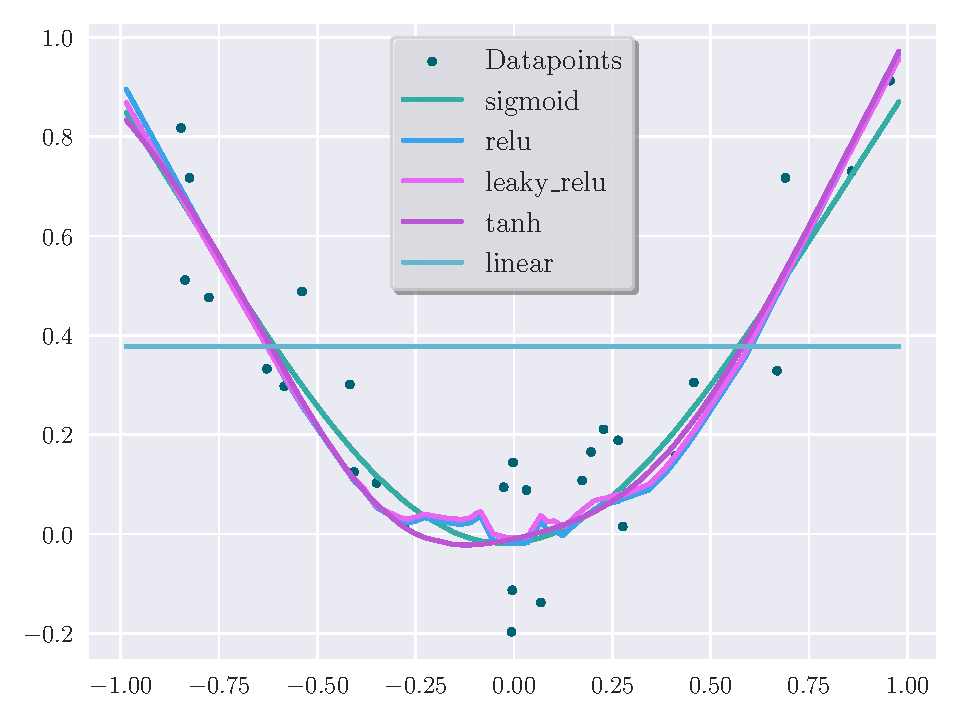
\includegraphics[width=\linewidth]{c_activations_2d_data.pdf}
                \caption{}
                \label[fig]{res:fig:act_funcs}
            \end{subfigure}
            \hfill 
            \begin{subfigure}{.49\textwidth}
                \centering
                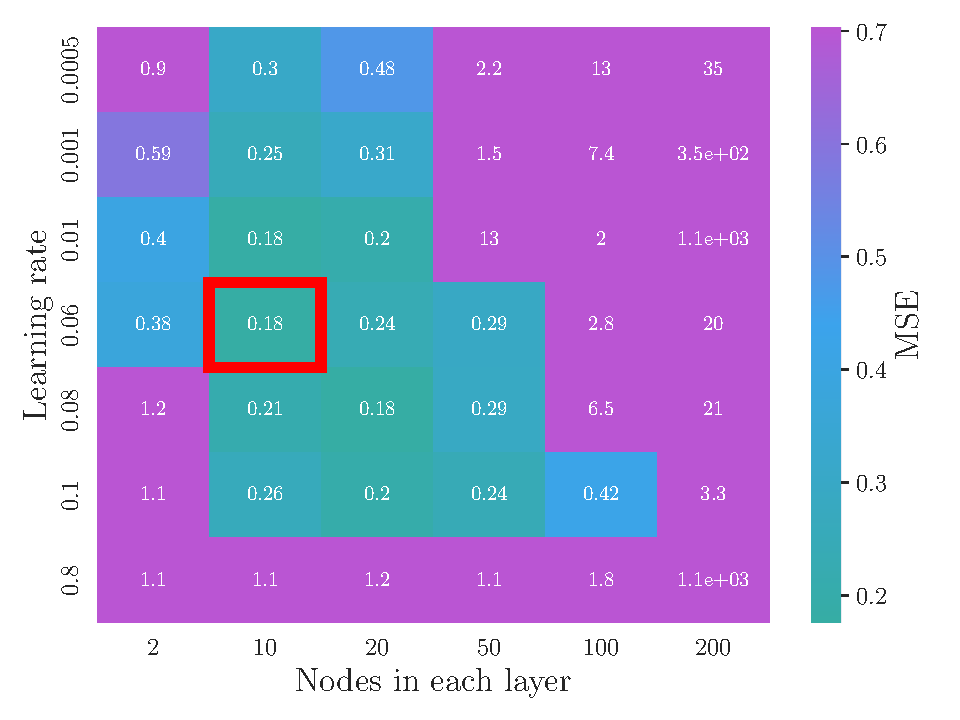
\includegraphics[width=\linewidth]{nodes_etas_heatmap_3_relu.pdf}
                \caption{}
                \label[fig]{res:fig:relu}
            \end{subfigure}
            \hfill 
            \begin{subfigure}{.49\textwidth}
                \centering
                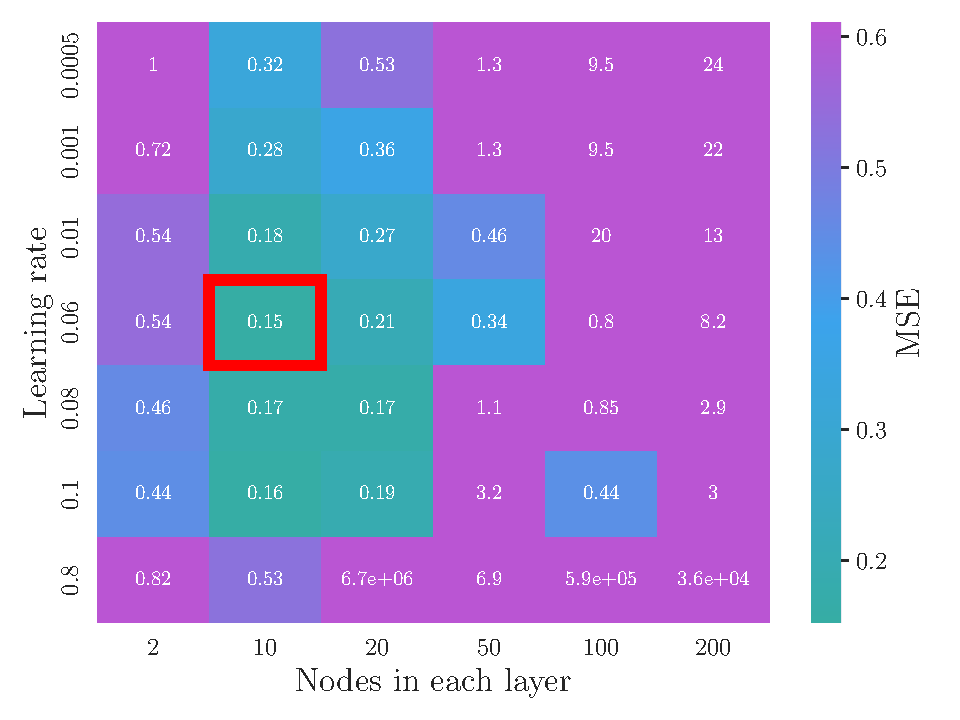
\includegraphics[width=\linewidth]{nodes_etas_heatmap_3_lrelu.pdf}
                \caption{}
                \label[fig]{res:fig:l_relu}
            \end{subfigure}
            \hfill 
            \begin{subfigure}{.49\textwidth}
                \centering
                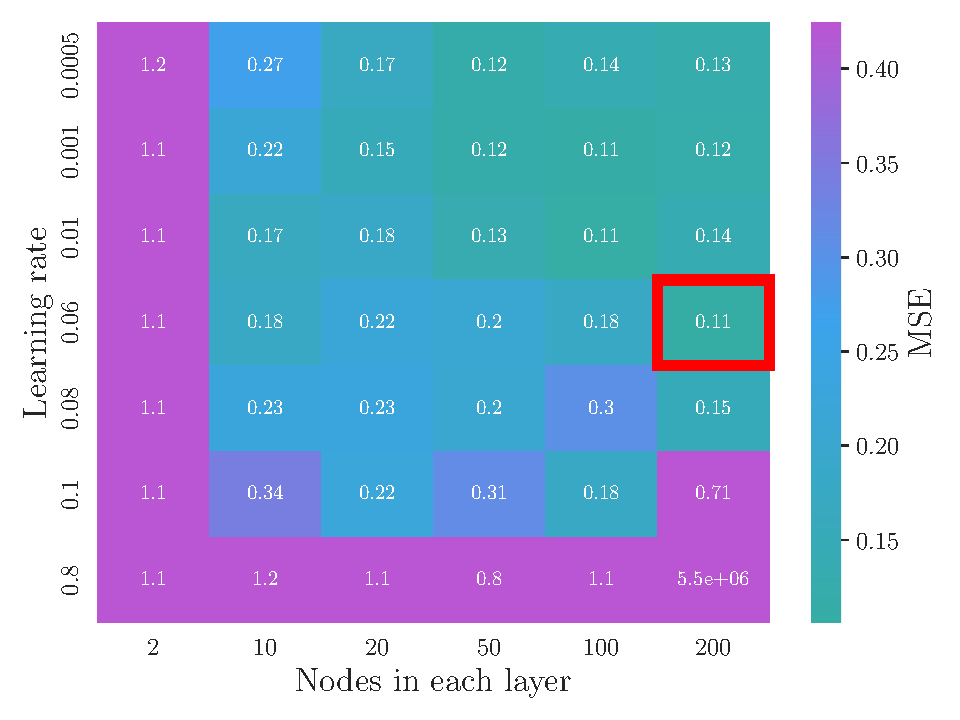
\includegraphics[width=\linewidth]{nodes_etas_heatmap_sk_3_relu.pdf}
                \caption{}
                \label[fig]{res:fig:sk_relu}
            \end{subfigure}
        \end{figure*}

    \subsubsection{Exploring Regularisation}
        % From $\lambda$ vs validation MSE-plot
        % Best MSE: 0.0782059642062313
        % corresponding lambda: 7.906043210907685e-05 or log10 of this: -4.102040816326531
        \begin{figure}
            \centering
            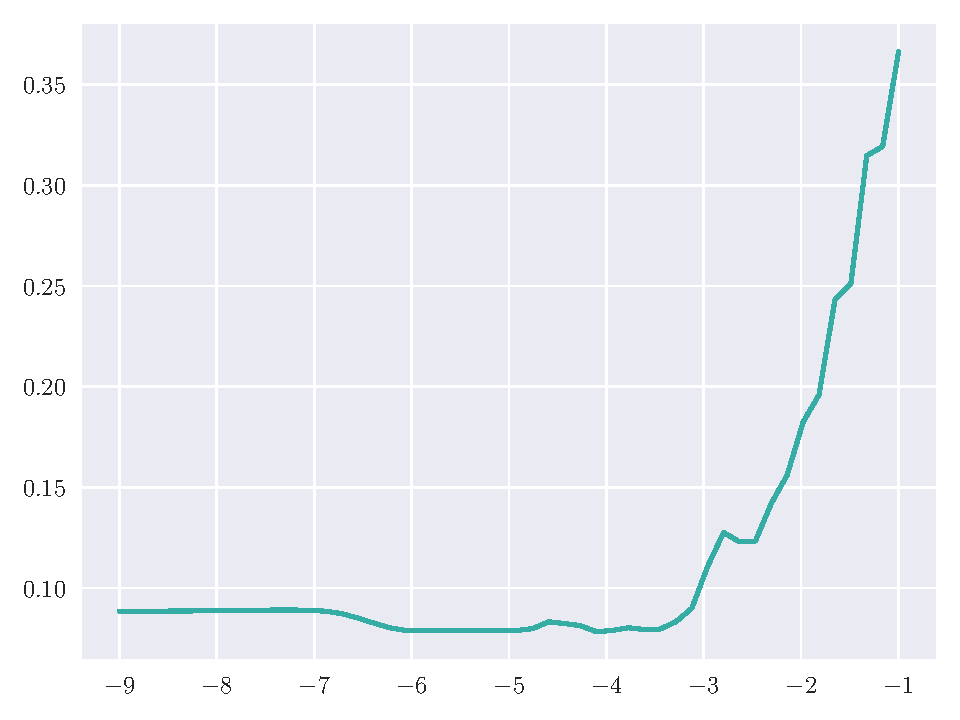
\includegraphics[width=\linewidth]{lmbdas_NN_reg.pdf}
            \caption{}
            \label[fig]{res:fig:regularisation}
        \end{figure}

    \subsubsection{Comparing with OLS}
        \begin{figure}
            \begin{subfigure}{.49\textwidth}
                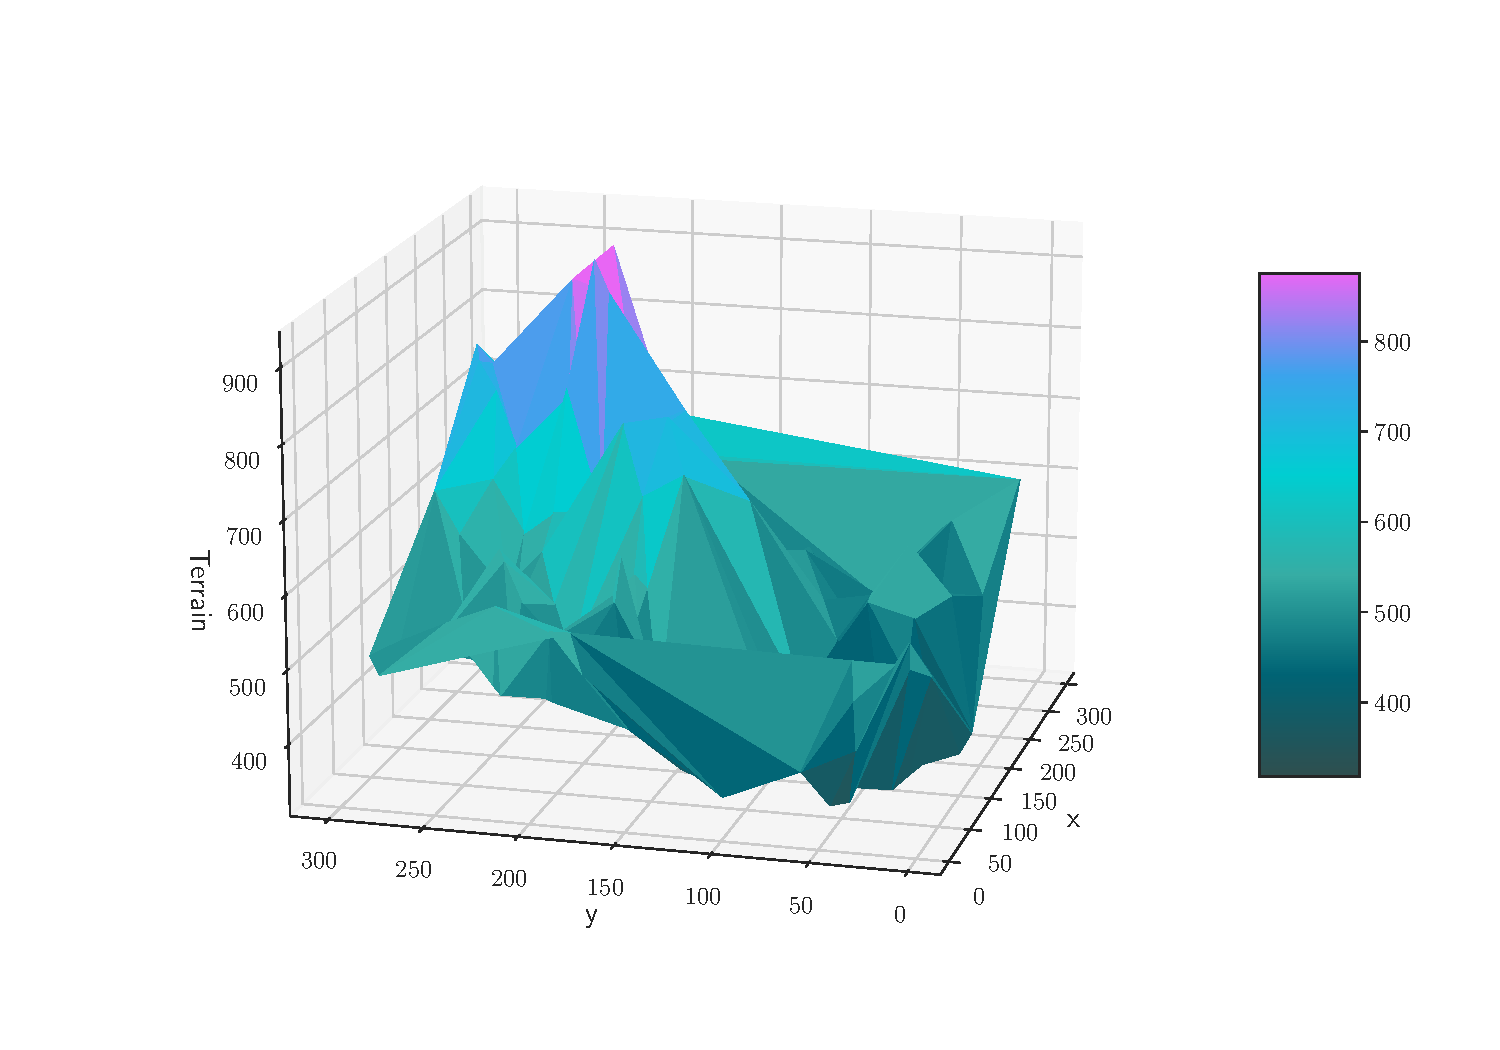
\includegraphics[width=\linewidth]{terrain_test.pdf}
                \caption{}
                \label[fig]{res:fig:terrain_test}
            \end{subfigure}
            \hfill 
            \begin{subfigure}{.49\textwidth}
                \centering
                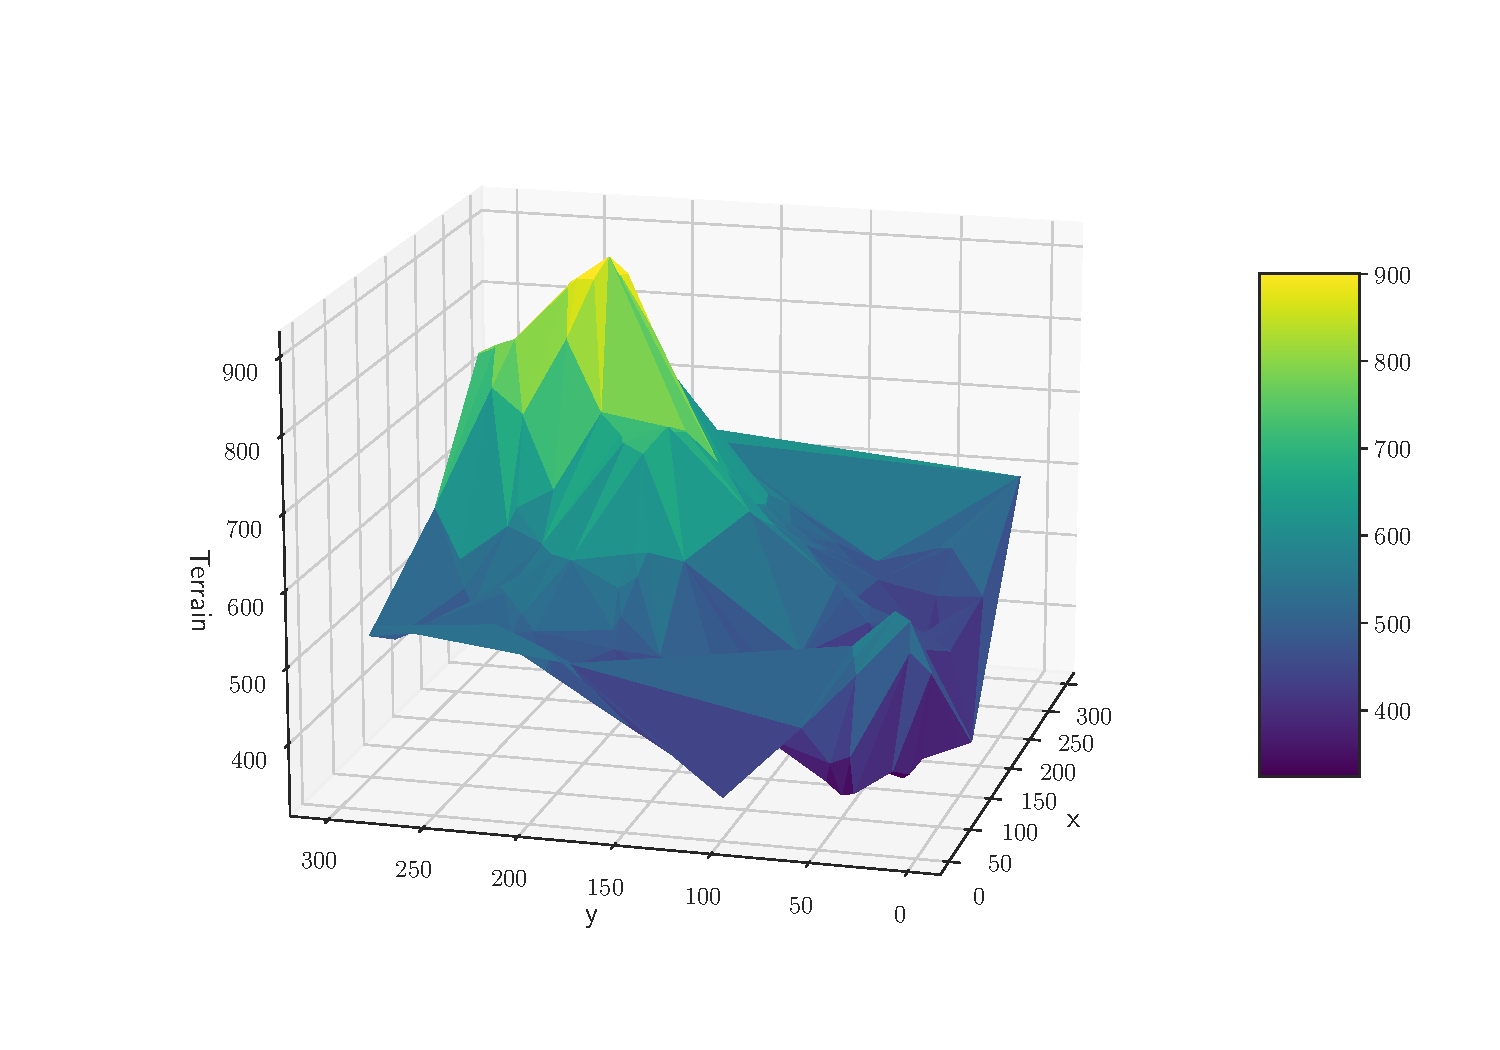
\includegraphics[width=\linewidth]{terrain_predicted.pdf}
                \caption{}
                \label[fig]{res:fig:terrain_pred_NN}
            \end{subfigure}
            \hfill 
            \begin{subfigure}{.49\textwidth}
                \centering
                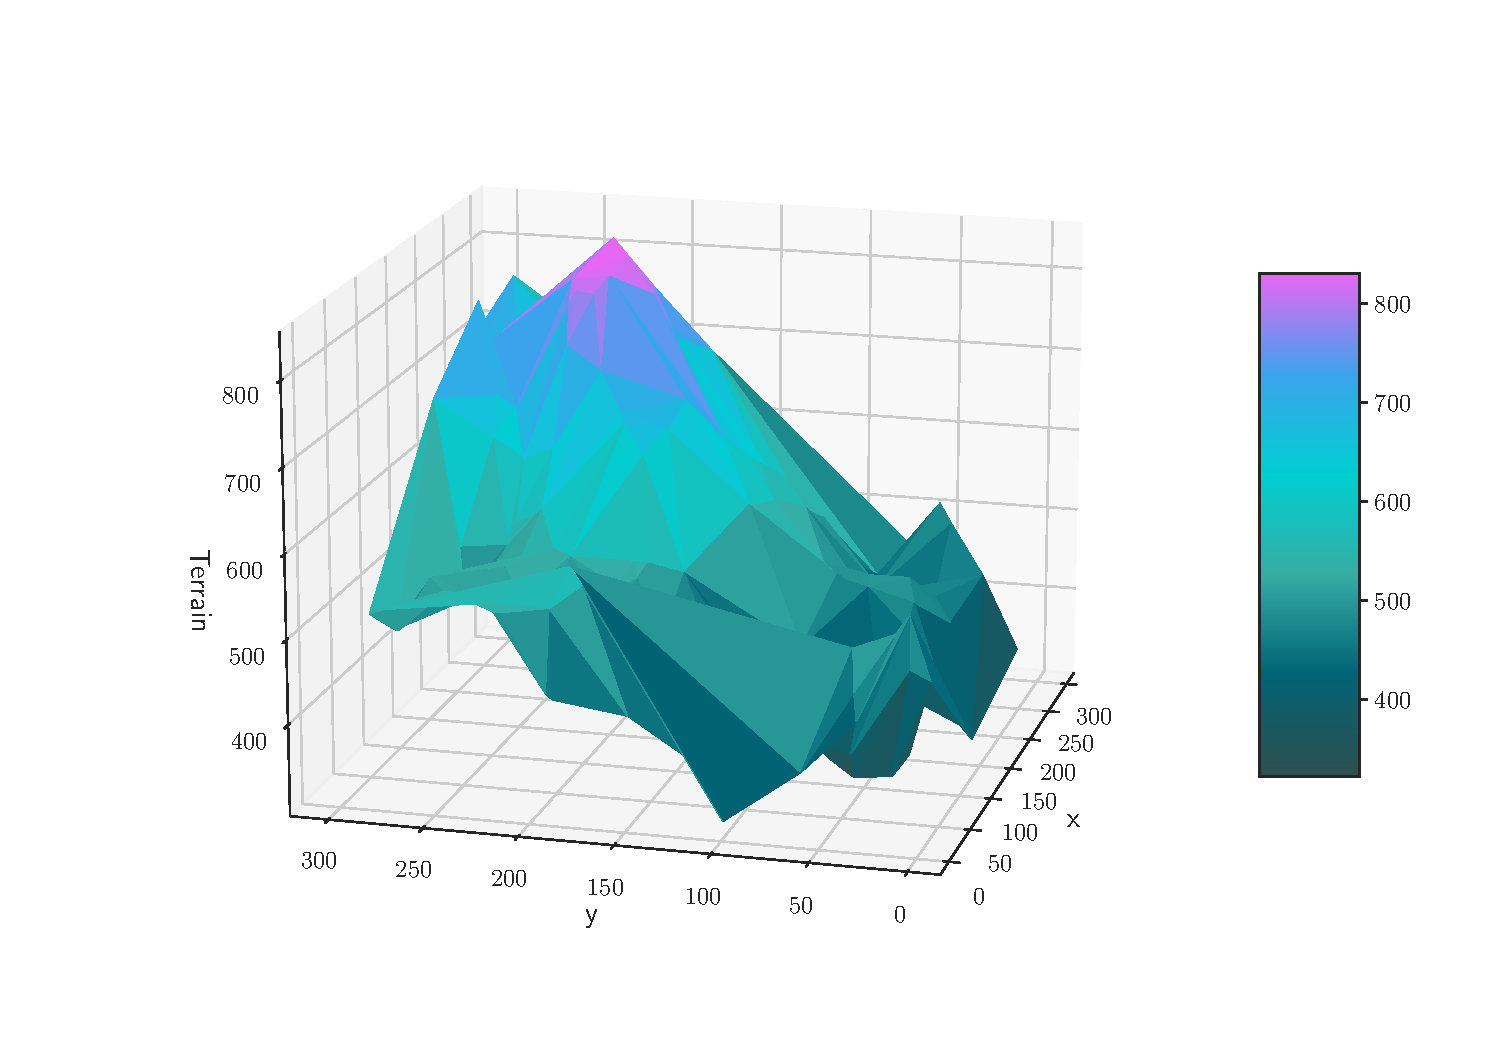
\includegraphics[width=\linewidth]{terrain_OLS.pdf}
                \caption{OLS MSE: 0.17086478937446714, $p=11$}
                \label[fig]{res:fig:terrain_pred_OLS}
            \end{subfigure}
        \end{figure}

    \comment{We have implemented a simple version of the models from Project 1 to get comparable results.}
        


\subsection{Wisconsin Breast Cancer}
    \subsubsection{Logistic regression}
    The different optimisation algorithms from our library of gradient decent methods were applied to optimise the BCE cost function without penalisation \cref{the:eq:logreg_cost_function} using Logistic regression. This is presented in \cref{res:fig:logreg_GD_opt} for GD methods with and without momentum, while SGD based methods is presented in \cref{res:fig:logreg_SGD_opt}.    

    \begin{figure}
        \begin{subfigure}{.49\textwidth}
            \centering
            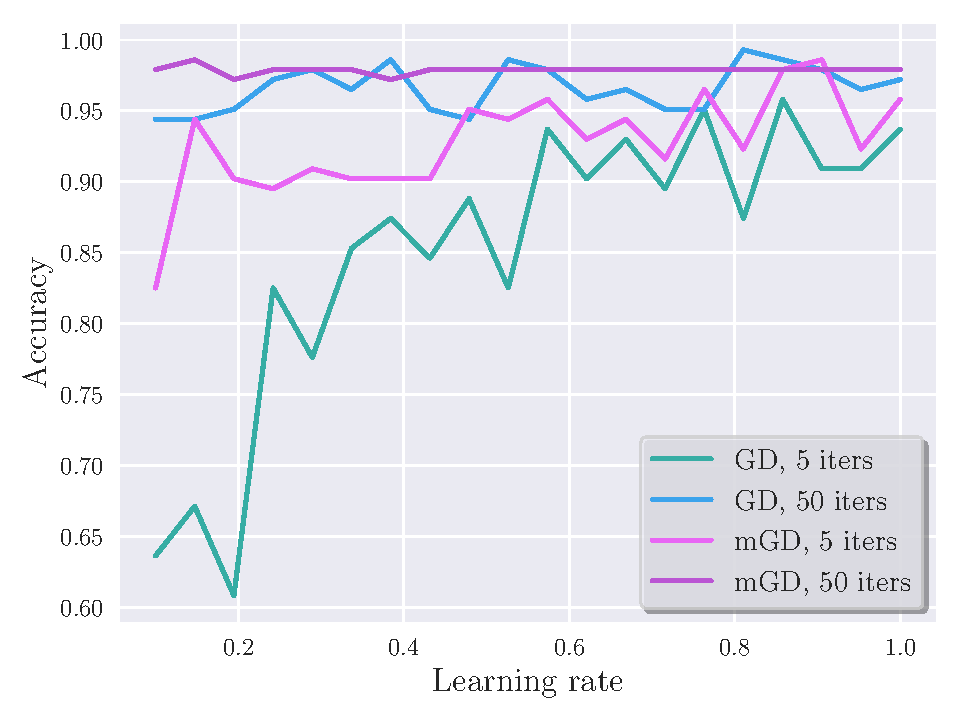
\includegraphics[width=\linewidth]{logreg_GD.pdf}
            \caption{Showing accuracy as a function of learning rate, optimised using GD with ($\gamma = 0.8$) and without momentum for 5 and 50 iterations.}
            \label[fig]{res:fig:logreg_GD_opt}
        \end{subfigure}
        \begin{subfigure}{.49\textwidth}
            \centering
            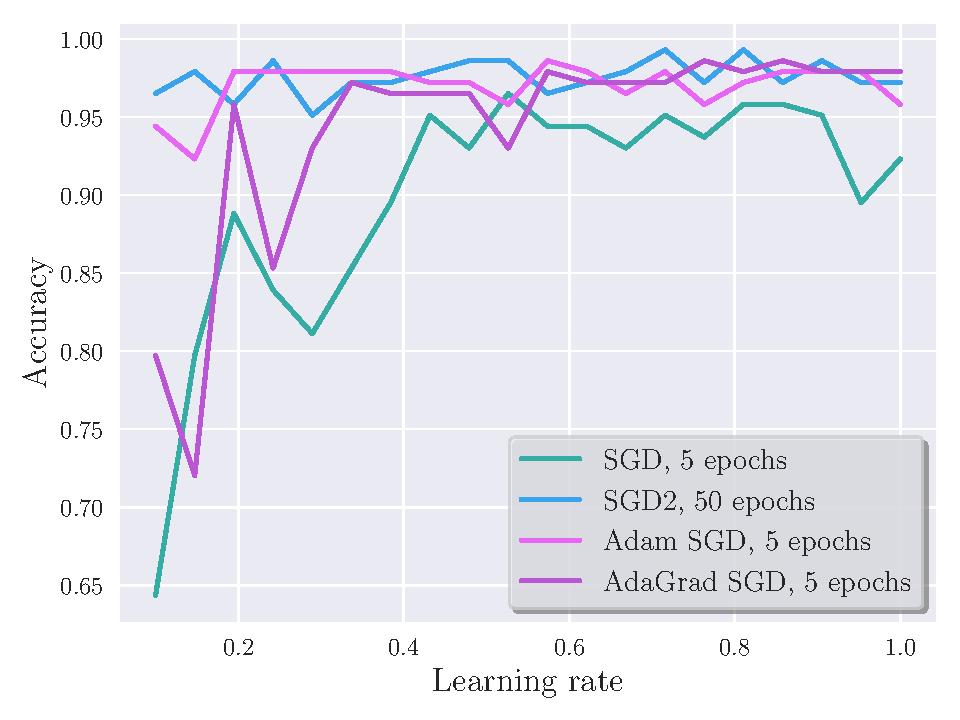
\includegraphics[width=\linewidth]{logreg_SGD.pdf}
            \caption{Showing accuracy as a function of learning rate, optimised plain, Adam ($\beta_1 = 0.9, \beta_2 = 0.99$) and AdaGrad SGD while varying the number of epochs. For all optimisations, a batch size of 200 was used.}
            \label[fig]{res:fig:logreg_SGD_opt}
        \end{subfigure}
        \begin{subfigure}{.49\textwidth}
            \centering
            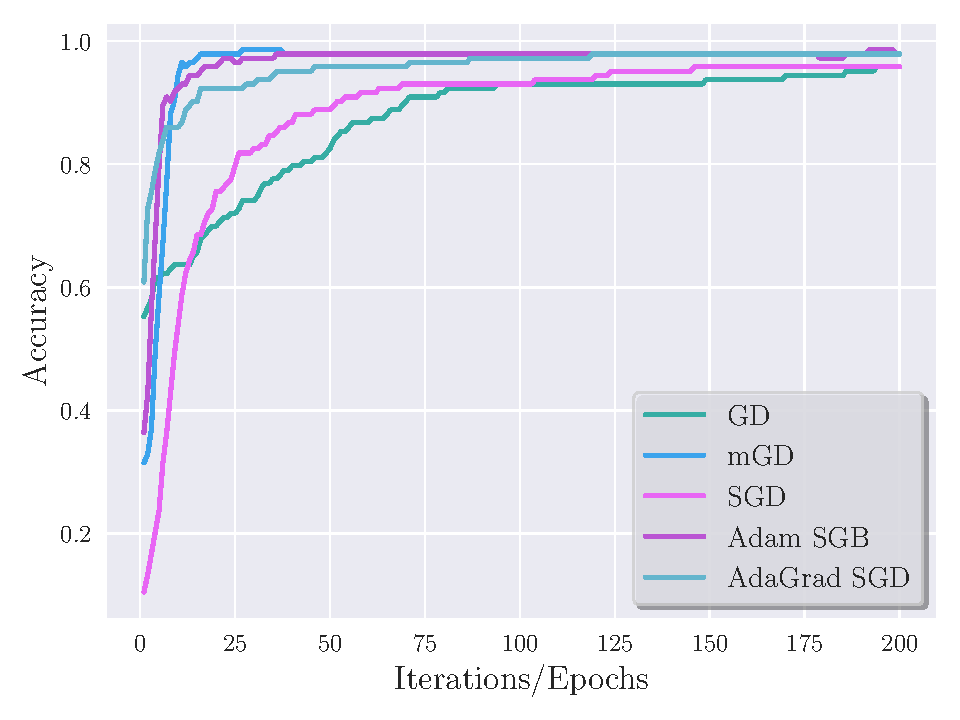
\includegraphics[width=\linewidth]{logreg_acc_during_optimazation.pdf}
            \caption{Showing accuracy as a function of iterations/epochs. All methods used $\eta = 0.05$, with Adam having $\beta_1 = 0.9, \beta_2 = 0.99$ and momentum GD $\gamma = 0.8$.}
            \label[fig]{res:fig:logreg_SGD_opt}
        \end{subfigure}
    \end{figure}

    \begin{figure*}
        \begin{subfigure}{.49\textwidth}
            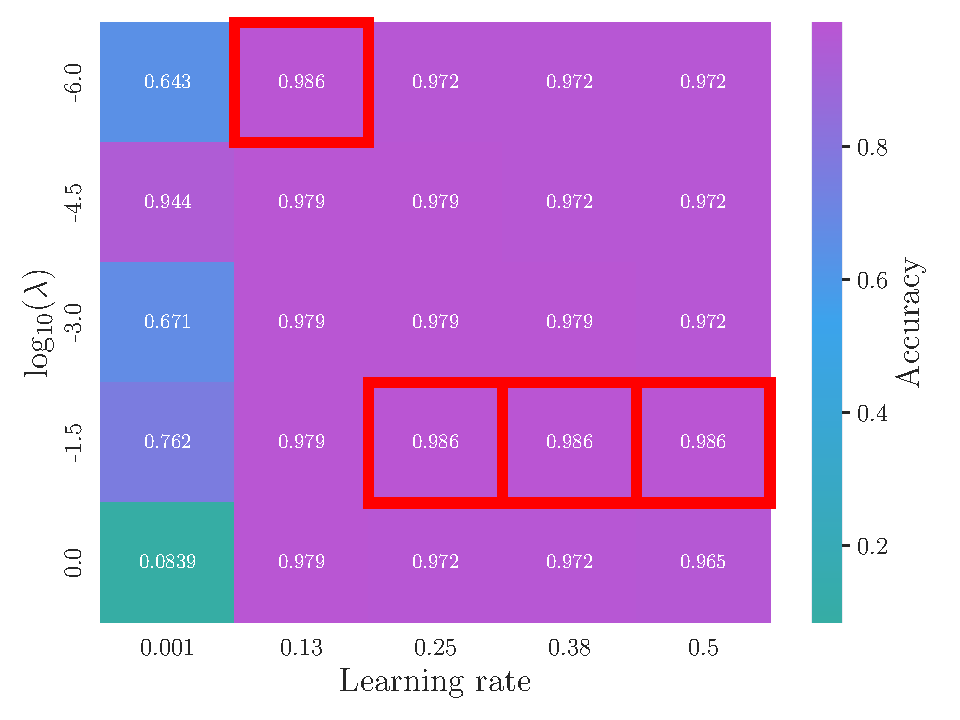
\includegraphics[width=\linewidth]{logreg_penalisation.pdf}
            \caption{Validation accuracy for logistic regression as a function of learning rate and penalisation parameter $\lambda$. Largest accuracy of $A = 0.986$ found at $\eta = 0.1, \lambda = 10^{-6}$.}
            \label[fig]{res:fig:logreg_penalisation_ours}
        \end{subfigure}
        \hfill 
        \begin{subfigure}{.49\textwidth}
            \centering
            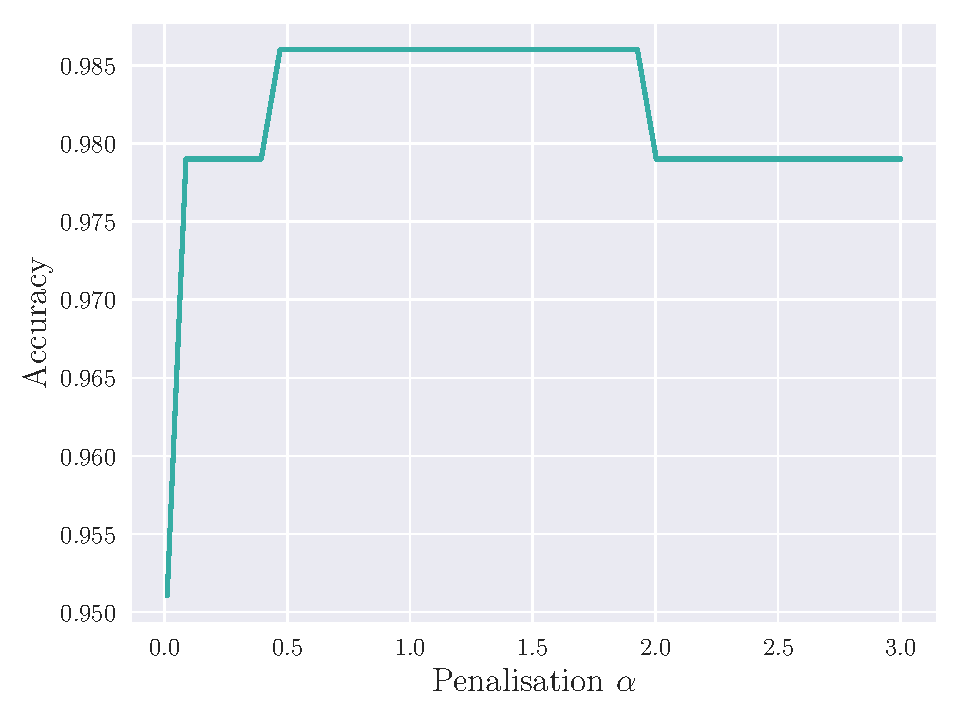
\includegraphics[width=\linewidth]{logreg_penalisation_sklearn.pdf}
            \caption{Validation accuracy for \textbf{scikit-learn}'s implementation of logistic regression as a function penalisation parameter $C$. }
            \label[fig]{res:fig:logreg_penalisation_sklearn}
        \end{subfigure}
        \caption{\comment{These plots are stupid, but I am tired and can not bother tweaking to make them look any better.}}
        \label[fig]{res:fig:logreg_penalisation}
    \end{figure*}

    \subsubsection{Classification Neural Network}
    \begin{table}
        \begin{tabular}{l|l|l|l|l}
            \network{1}{5} & \network{1}{10} & \network{2}{5} & \network{3}{5} & $f_H$       \\
            \hline
            0.993             & 0.986              & 0.993             & 0.993             & Sigmoid    \\
            0.993             & 0.986              & 0.993             & 0.993             & Tanh       \\
            0.979             & 0.979              & 0.986             & 0.979             & ReLU       \\
            0.979             & 0.986              & 0.979             & 0.979             & Leaky ReLU
        \end{tabular}
        \caption{The optimal validation accuracy scores calculated using different network structures and hidden activation functions $f_H$, across different learning rates. Multiple learning rates correspond to the same accuracy score.}
        \label[tab]{res:tab:accuracy_score_activation_functions}        
    \end{table}

    \begin{figure*}
        \begin{subfigure}{.49\textwidth}
            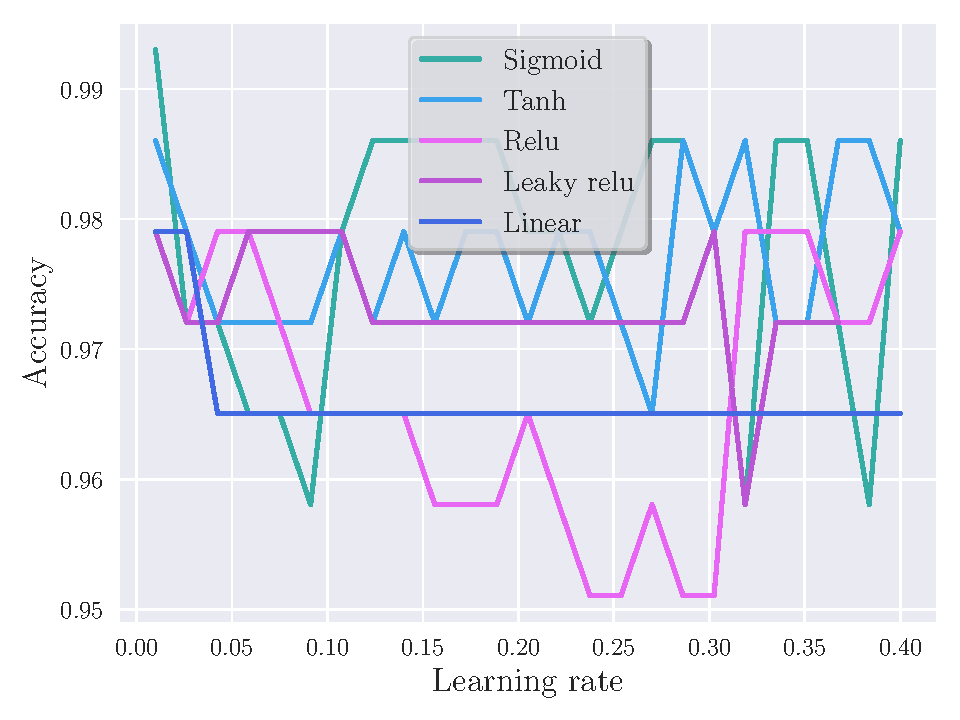
\includegraphics[width=\linewidth]{clasf_activation_functions1.pdf}
            \caption{Network \network{1}{5}, plotted for $\eta \in [ 0.01, 0.4 ]$ using 8 linearly spaced points}
            \label[fig]{res:fig:clf_af_N_1_5}
        \end{subfigure}
        \hfill 
        \begin{subfigure}{.49\textwidth}
            \centering
            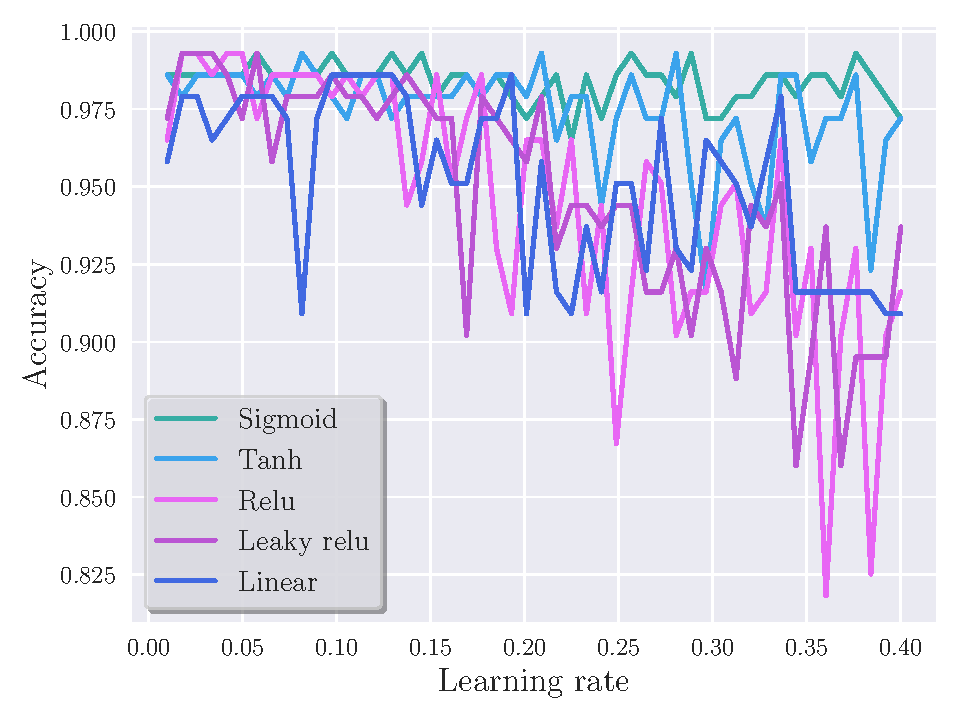
\includegraphics[width=\linewidth]{clasf_activation_functions2.pdf}
            \caption{Network \network{1}{10}, plotted for $\eta \in [ 0.001, 0.01 ]$ using 8 linearly spaced points}
            \label[fig]{res:fig:clf_af_N_1_10}
        \end{subfigure}
        \hfill 
        \begin{subfigure}{.49\textwidth}
            \centering
            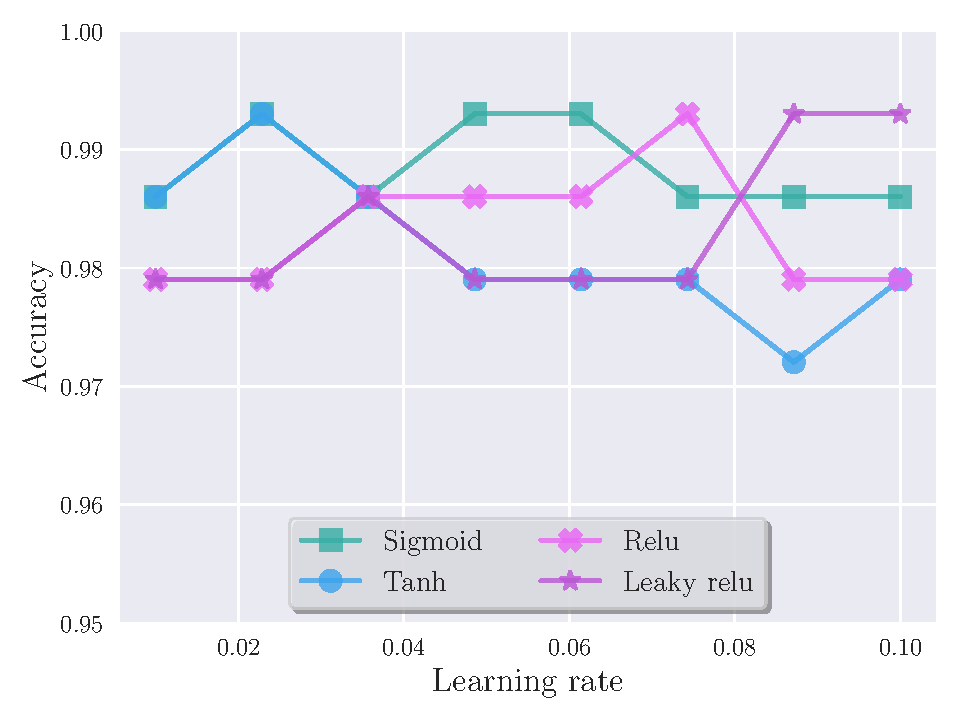
\includegraphics[width=\linewidth]{clasf_activation_functions3.pdf}
            \caption{Network \network{2}{5}, plotted for $\eta \in [ 0.001, 0.01 ]$ using 8 linearly spaced points}
            \label[fig]{res:fig:clf_af_N_2_5}
        \end{subfigure}
        \hfill 
        \begin{subfigure}{.49\textwidth}
            \centering
            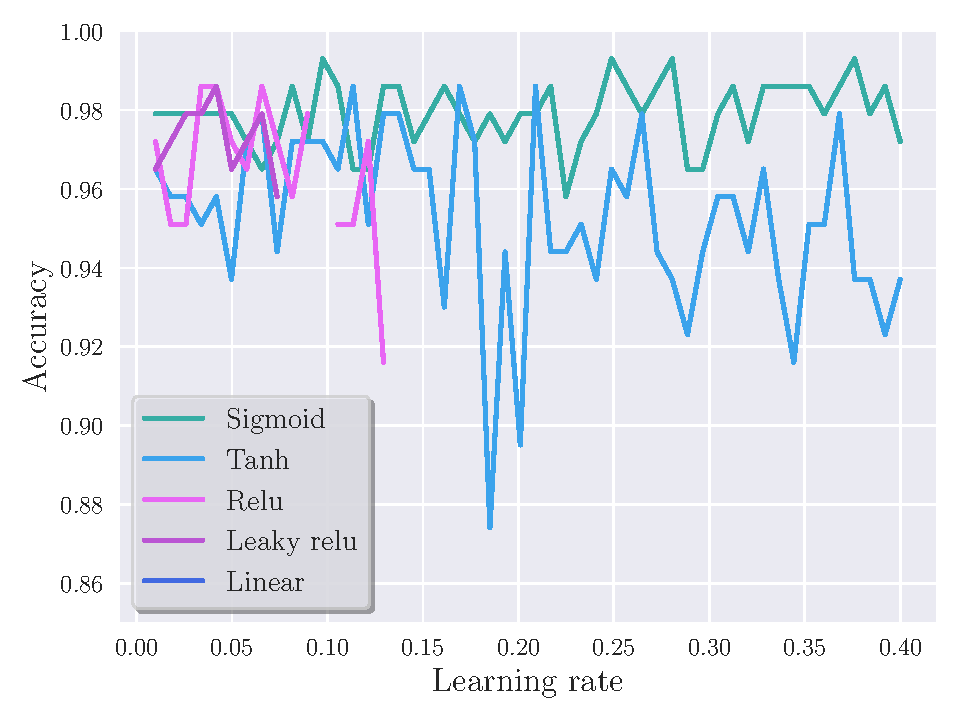
\includegraphics[width=\linewidth]{clasf_activation_functions4.pdf}
            \caption{Network \network{3}{5}, plotted for $\eta \in [ 0.001, 0.01 ]$ using 8 linearly spaced points}
            \label[fig]{res:fig:clf_af_N_3_5}
        \end{subfigure}
        \caption{Plots of the accuracy score against learning rate for different activation functions for used for the hidden layer(s). Different network models have been used for the four plots. The AdaGrad algorithm with momentum $\gamma = 0.8$ has been used for optimisation, running 100 epochs with a batch size of 200.}
        \label[fig]{res:fig:clf_afs}
    \end{figure*}

    \begin{figure*}
        \begin{subfigure}{.49\textwidth}
            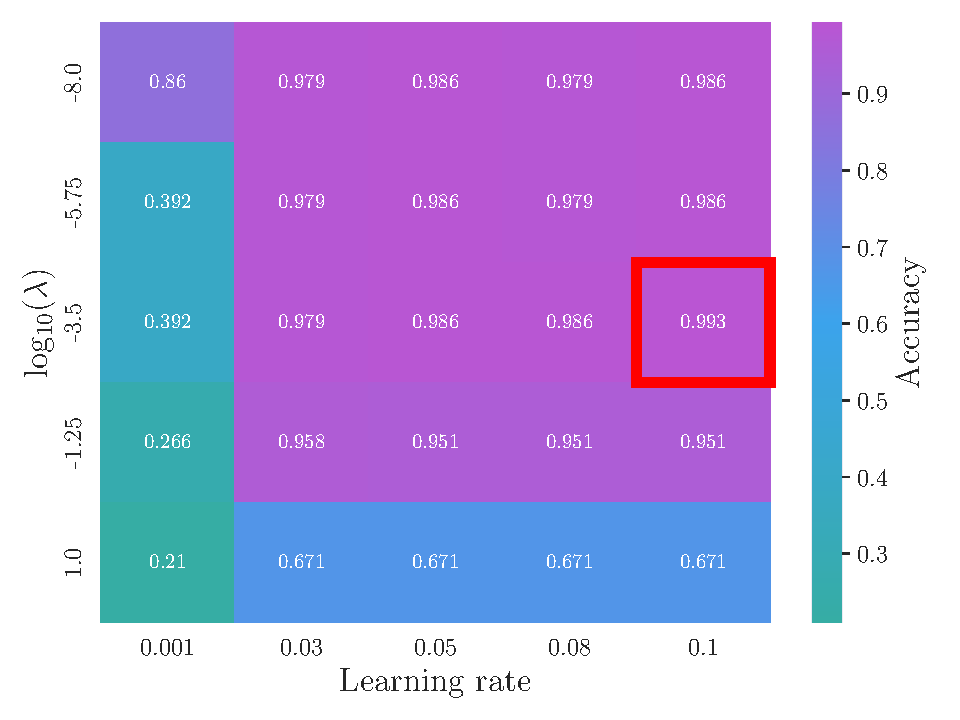
\includegraphics[width=\linewidth]{lmbda_lr_struct0_sigmoid.pdf}
            \caption{Network \network{1}{5} with a Sigmoid activation function for the hidden layer. A single maximum was found with an accuracy $A = 0.993$, using $\eta = 0.1$ and $\lambda = 10^{-3.5}$}
            \label[fig]{res:fig:clf_heatmap_N_1_5_sig}
        \end{subfigure}
        \hfill
        \begin{subfigure}{.49\textwidth}
            \centering
            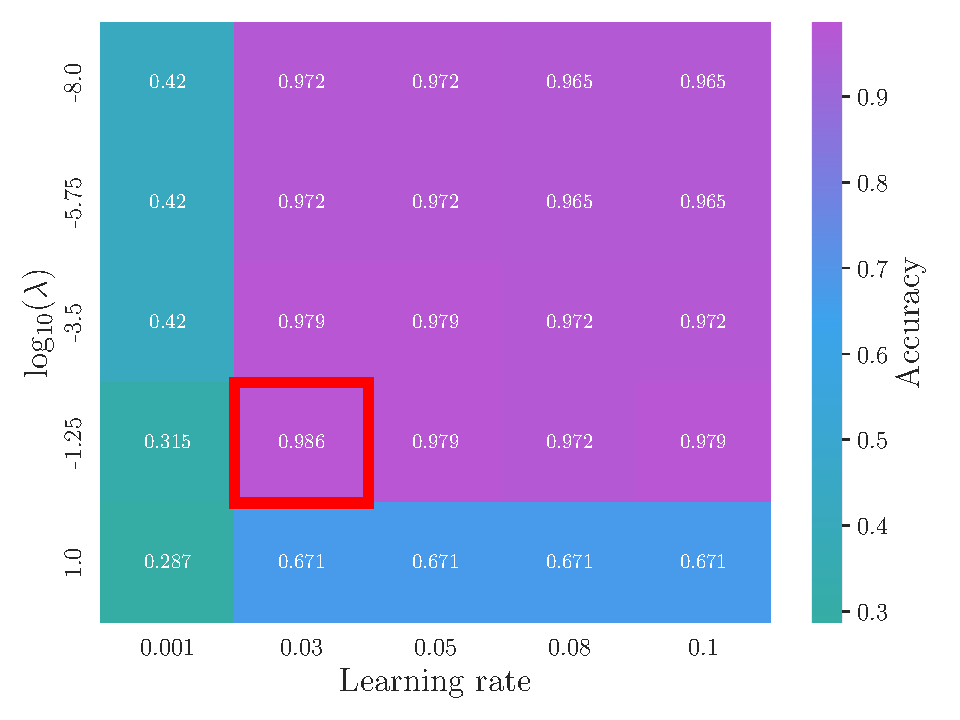
\includegraphics[width=\linewidth]{lmbda_lr_struct0_tanh.pdf}
            \caption{Network \network{1}{5} with a Hyperbolic tangent activation function for the hidden layer. A single maximum was found with an accuracy $A = 0.986$, using $\eta = 0.03$ and $\lambda = 10^{-1.25}$}
            \label[fig]{res:fig:clf_heatmap_N_1_5_tanh}
        \end{subfigure}
        \hfill
        \begin{subfigure}{.49\textwidth}
            \centering
            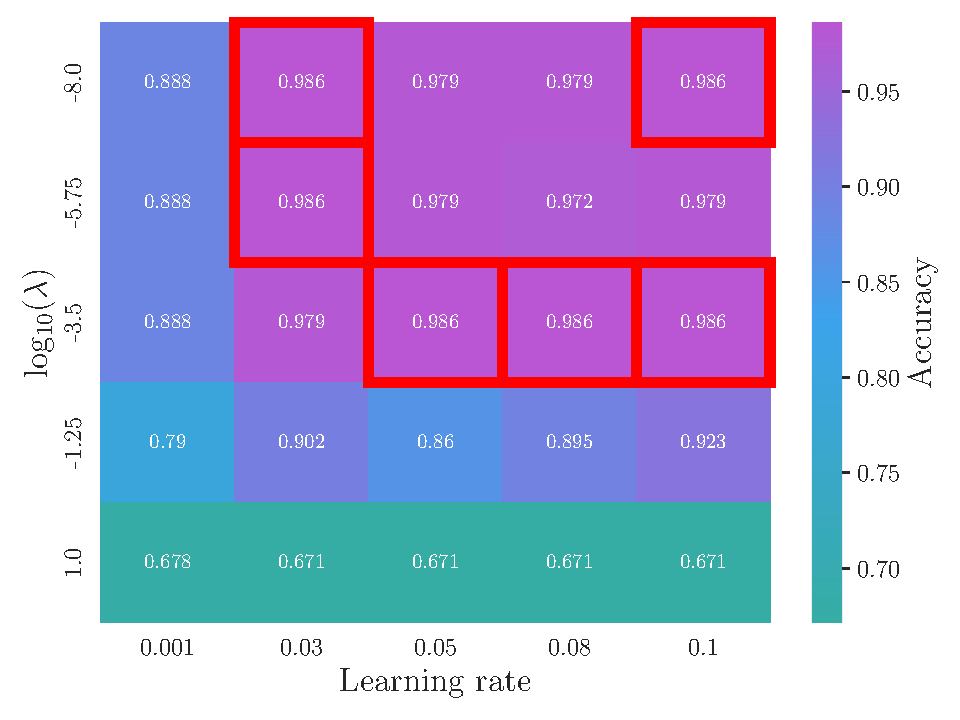
\includegraphics[width=\linewidth]{lmbda_lr_struct1_sigmoid.pdf}
            \caption{Network \network{2}{5} with a Sigmoid activation function for the hidden layers. Multiple maxima was found with an accuracy $A = 0.986$.}
            \label[fig]{res:fig:res:fig:clf_heatmap_N_2_5_sig}
        \end{subfigure}
        \hfill
        \begin{subfigure}{.49\textwidth}
            \centering
            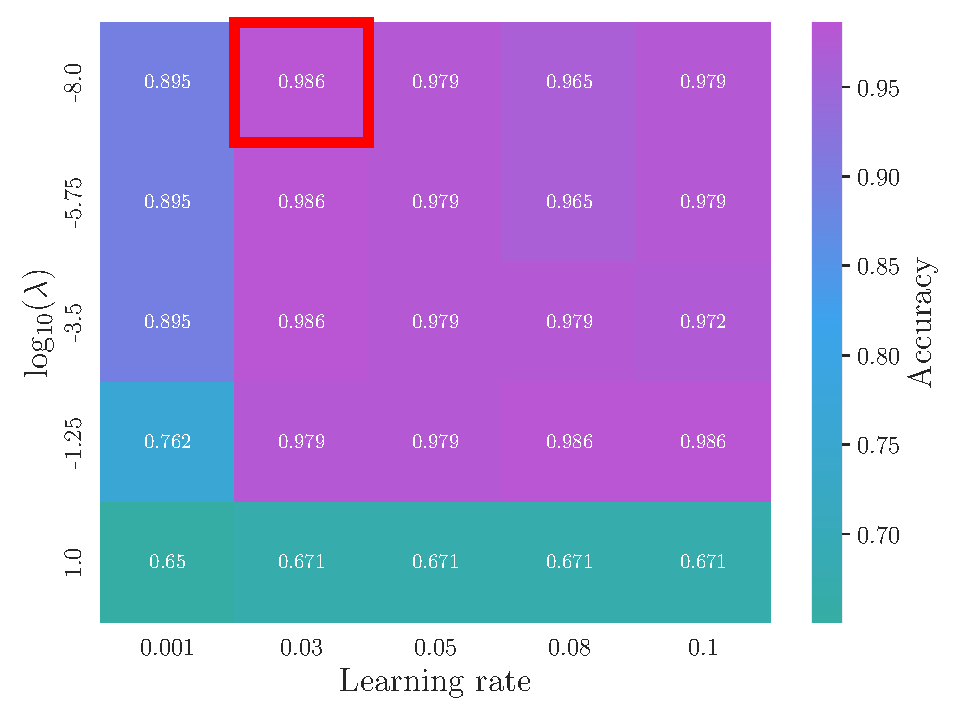
\includegraphics[width=\linewidth]{lmbda_lr_struct1_tanh.pdf}
            \caption{Network \network{2}{5} with a Hyperbolic activation function for the hidden layers. Multiple maxima was found with an accuracy $A = 0.986$.}
            \label[fig]{res:fig:clf_heatmap_N_2_5_tanh}
        \end{subfigure}
        \caption{Plots of validation accuracy score varied against learning rate and penalisation term $\lambda$. Red squares mark the best accuracy scores. The first row contains the network structures \network{1}{5} with Sigmoid (a) and Hyperbolic tangent (b) activation functions for the output layer, while the second row contains \network{2}{5} with Sigmoid (a) and Hyperbolic tangent (b). The AdaGrad algorithm with momentum $\gamma = 0.8$ has been used for optimisation, running 100 epochs with a batch size of 200.}
        \label[fig]{res:fig:clf_heatmaps}
    \end{figure*}


    \subsubsection{SKLERN STUFF}
    \begin{figure}
        \centering
        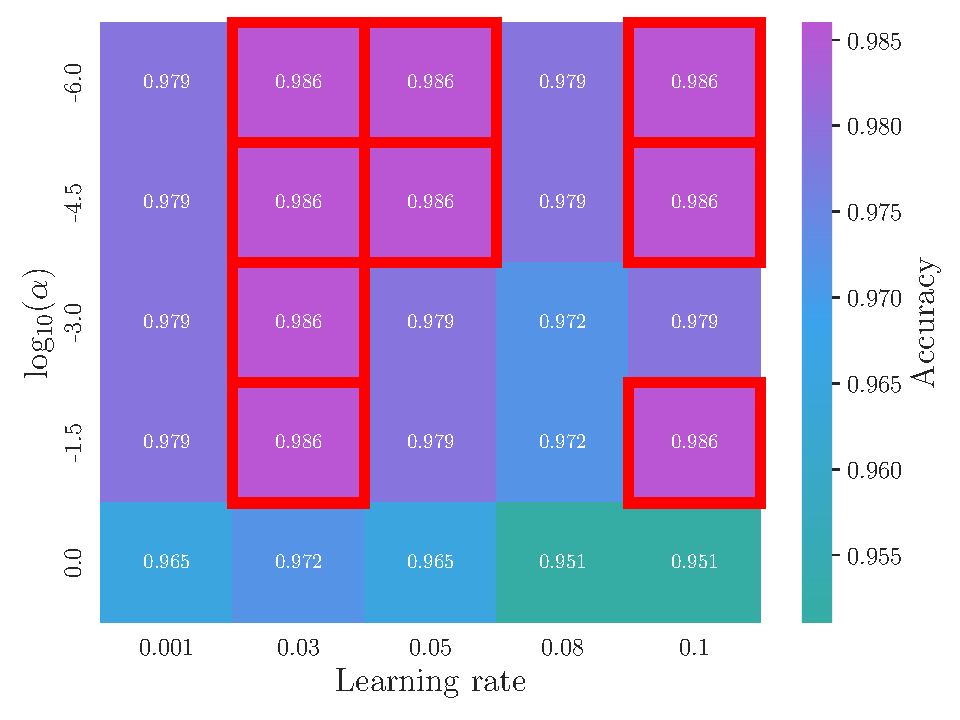
\includegraphics[width=\linewidth]{alpha_lr_struct1_sigmoid_sklearn.pdf}
        \caption{sklearn \network{2}{5}}
    \end{figure}